\documentclass{standalone}

\usepackage{tikz}
\usetikzlibrary{positioning, calc}

\begin{document}
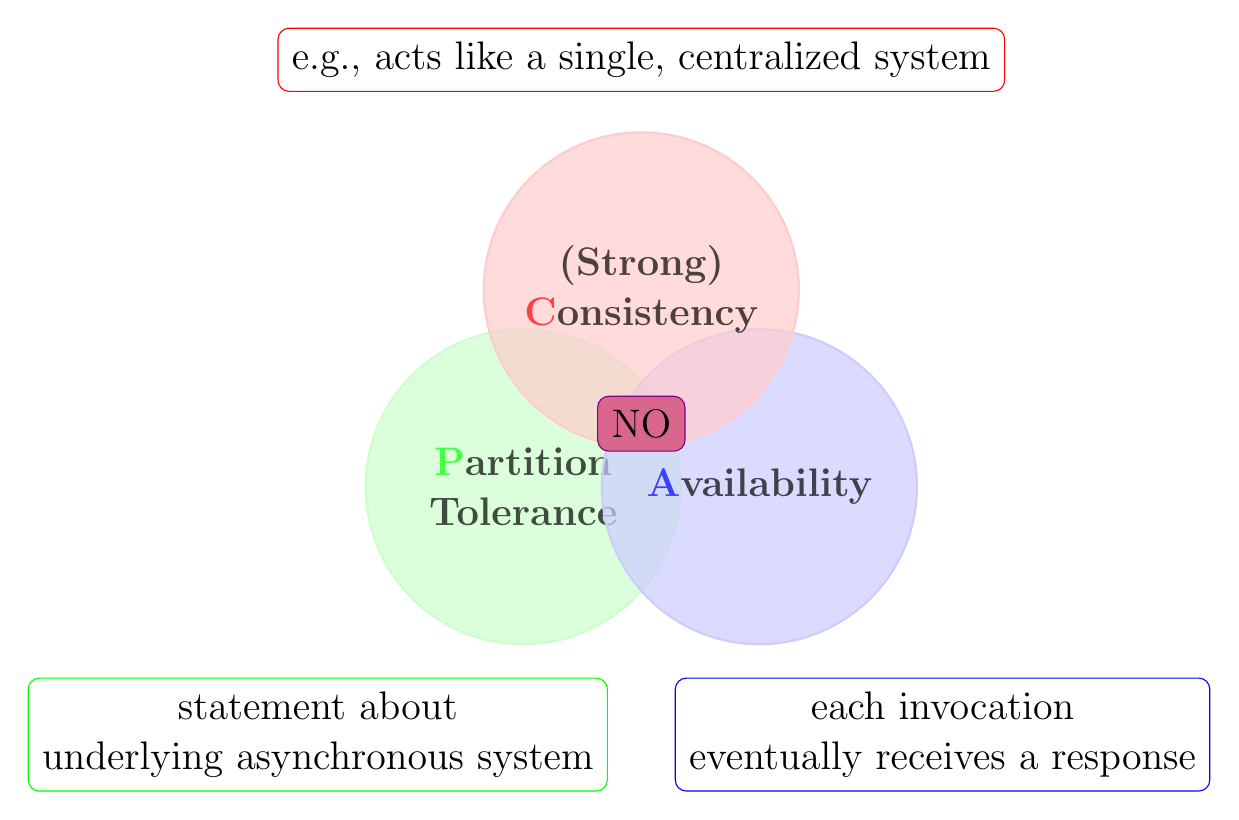
\begin{tikzpicture}[qnode/.style = {circle, minimum size = 4.0cm, font = \Large, thick, draw = #1, align = center, fill = #1, fill opacity = 0.70}]
  \node (p) [qnode = green!20] at (0,0) {\bf \textcolor{green}{P}artition \\ \bf Tolerance};
  \node (a) [qnode = blue!20] at (3.0,0) {\bf \textcolor{blue}{A}vailability};
  \node (c) [qnode = red!20] at (1.5, 2.5) {\bf (Strong) \\ \bf \textcolor{red}{C}onsistency};
  
  \node (no) [rectangle, draw, fill = purple!60, draw = violet, font = \Large, inner sep = 5pt, rounded corners] at (1.5, 0.8) {NO};
  
  \begin{scope}[txt/.style = {font = \Large, align = center, rectangle, draw = #1, rounded corners, 
    inner sep = 5pt}]
    \node (ctxt) [txt = red, above = 0.5cm and 0.cm of c, font = \Large] {e.g., acts like a single, 
    centralized system};
    \node (atxt) [txt = blue, below right = 1.0cm and -2.5cm of a, font = \Large] {each invocation 
    \\ eventually receives a response};    \node (ptxt) [txt = green, below left = 1.0cm and -2.5cm 
    of p, font = \Large] {statement about \\ underlying asynchronous system};        
  \end{scope}
\end{tikzpicture}
\end{document}
